\documentclass[tikz,border=10pt]{standalone}
\begin{document}
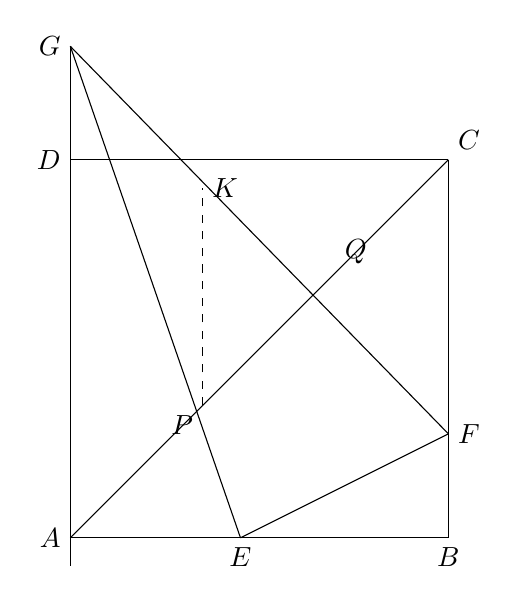
\begin{tikzpicture}[scale=1.2]
\coordinate (A) at (0,0);
\coordinate (B) at (4,0);
\coordinate (C) at (4,4);
\coordinate (D) at (0,4);
\coordinate (E) at (1.8,0);
\coordinate (F) at (4,1.1);
\coordinate (G) at (0,5.2);
\coordinate (P) at (1.4,1.4);
\coordinate (Q) at (2.8,2.8);
\coordinate (K) at (1.4,3.7);

\draw (G) -- (D) -- (0,-0.3);
\draw (D) -- (C);
\draw (A) -- (E);
\draw (E) -- (B) -- (C);
\draw (A) -- (C);
\draw (G) -- (F);
\draw (G) -- (E);
\draw (E) -- (F);
\draw[dashed] (P) -- (K);

\node[left] at (A) {$A$};
\node[below] at (B) {$B$};
\node[above right] at (C) {$C$};
\node[left] at (D) {$D$};
\node[below] at (E) {$E$};
\node[right] at (F) {$F$};
\node[left] at (G) {$G$};
\node[below left] at (P) {$P$};
\node[above right] at (Q) {$Q$};
\node[right] at (K) {$K$};
\end{tikzpicture}
\end{document}
